\documentclass[a4paper, 12pt]{ppgeb}

% |--- Títulos, autor, banca ---|----------------------{{{
% Autor:
% Substituta  as informações nos comandos a seguir, até a linha começando
% com \membrobancaexterno.
% Em \title: título na forma principal, como aparecerá em algumas páginas
% Em \tituloficha: título como aparecerá na ficha catalográfica; idêntico
% ao anterior, mas com possíveis quebras manuais de linha (usar \\ quando
% necessário, para ajustar as mudanças de linha na ficha catalográfica).
% Em   \titulocapaA,   \titulocapaB,   \titulocapaC:  título para a capa,
% dividido em no  máximo 3  linhas (coloque uma  linha em  cada  comando,
% dividindo como ficar melhor esteticamente).
% Remova  o  símbolo  de  comentário  (%)  de  \coorientador,  se  houver
% coorientador.
%  Em  \publicacao{011A/2019}:  o  número  final  será   fornecido   pela

\title{Coleta Simultânea de Eletroencefalograma \\ e Rastreamento Ocular: Ferramenta e Estudo de Caso}
\tituloficha{Coleta Simultânea de Eletroencefalograma e Rastreamento Ocular: Ferramenta e Estudo de Caso\\\phantom{}[Distrito Federal], 2019.} 
\titulocapaA{Coleta Simultânea de Eletroencefalograma e}
\titulocapaB{e Rastreamento Ocular: Ferramenta e Estudo de Caso}
\titulocapaC{}
\titulofichadois{Coleta Simultânea de Eletroencefalograma e Rastreamento Ocular: Ferramenta e Estudo de Caso}
\author{Ana Paula Sandes de Souza}
\nomeinvertido{Souza, Ana}
\orientador{Dr. Gerardo Antonio Idrobo Pizo}
%\coorientador{Nome do Coorientador}
\publicacao{011A/2022}
\data{Agosto de 2022}
\ano{2022}
\areaum{Neurociência Computacional} % Preencher com termos escolhidos para identificar a área
\areadois{Eletroencefalograma}
\areatres{Rastreamento Ocular}
\areaquatro{Sincronização de Sinais}
\endereco{anapaulasandes.s@gmail.com}
\cep{CEP 73105-904}

\membrobancainterno{DRª. Marília Miranda Forte Gomes}
\membrobancaexterno{Dr. Membro Externo}
%---}}}

% |--- Bibliotecas utilizadas ---|----------------------{{{
\usepackage[margin=1in]{geometry}
\usepackage{setspace}
\usepackage{multirow}
\usepackage{booktabs}
 \usepackage[brazil]{babel}
\usepackage{xfrac}
\usepackage{hyperref}
\hypersetup{
colorlinks = true,
linkcolor = black,
anchorcolor = blue,
citecolor = blue,
filecolor = blue,
urlcolor = blue
}
\usepackage{rotating}
\usepackage[margin=0.40in,font=small,labelfont=bf,labelsep=period]{caption}
%---}}}

% |- Formato de referências (use apenas uma das 2 linhas seguintes; comente a outra) -|-{{{
\newcommand{\formatobibliografia}{numero}
%\newcommand{\formatobibliografia}{autorano}

\ifthenelse{\equal{\formatobibliografia}{numero}}{
\bibliographystyle{plain}
}
{}

\ifthenelse{\equal{\formatobibliografia}{autorano}}{
\usepackage{apalike}
\bibliographystyle{apalike}
}
{}
%---}}}

% |--- Espaçamento, configuração de título de seções ---|----------------------{{{
\onehalfspacing

\makeatletter
\renewcommand{\section}{\@startsection
{section}
{1}
{0mm}
{-\baselineskip}
{0.5\baselineskip}
{\large\bfseries\scshape}}
\makeatother

\makeatletter
\renewcommand{\subsection}{\@startsection
{subsection}
{2}
{0mm}
{-\baselineskip}
{0.5\baselineskip}
{\bf\sffamily}}
\makeatother

\makeatletter
\renewcommand{\subsubsection}{\@startsection
{subsubsection}
{3}
{0mm}
{-\baselineskip}
{0.5\baselineskip}
{\bf\sffamily}}
\makeatother

\setlength{\parindent}{20pt}
\setlength{\parskip}{06pt}
\newcommand{\spaceinitialsname}{0.4mm}
\newcommand{\porcento}{\scalebox{0.5}{~}\scalebox{0.9}{\%}}
\newcommand{\scanner}{\emph{scanner}}
\newcommand{\scanners}{\emph{scanners}}
\newcommand{\cmcubico}{${\textrm{cm}^{\scalebox{0.7}{3} }}$}
\setcounter{secnumdepth}{3}
%\setcounter{tocdepth}{3}
%---}}}

% |--- Comandos especiais ---|----------------------{{{
\newcommand{\cmquad}{${\textrm{cm}^{\scalebox{0.7}{2}} }$}
\newcommand{\mmquad}{${\textrm{mm}^{\scalebox{0.7}{2}} }$}
\newcommand{\gcmquad}{${\textrm{g}}/{\textrm{cm}^{\scalebox{0.7}{2}} }$}
\newcommand{\subsecref}[1]{Seção~\ref{#1}}
\newcommand{\figref}[1]{Figura~\ref{#1}}
\newcommand{\etal}{\emph{et~al.}}
\newcommand{\Jawsonly}{{\emph{Jaws-Only}} }
\newcommand{\jawsonly}{{\emph{jaws-only}} }
\newcommand{\software}{\emph{software}}
\newcommand{\percentagesignscale}{0.8}
\newcommand{\percent}{\scalebox{\percentagesignscale}{~\%}}
\newcommand{\subsubsubsection}[1]{\vspace{16pt}\noindent\textbf{#1}\\[12pt]}
%---}}}

% |--- Diretório(s) com figuras (se desejar, inclua subdiretórios) ---|-------------{{{
\graphicspath{{figuras/}}
%---}}}

% |--- Lista de palavras que não podem ser separadas em sílabas ---|------------------{{{
\hyphenation{development results Commissioning possibility Philadelphia Devic Calculations Calculation Language}
%---}}}

% |--- Texto principal ---|----------------------{{{
\begin{document}

\maketitle

% Se desejar uma epígrafe, remova o % do início das próximas linhas (até ==============)
%\clearpage
%\hspace{1mm}
%
%\vfill
%
%\hspace{1mm}
%
%\begin{center}
%\emph{Epígrafe} \\
%Autor da epígrafe
%\end{center}
%
%\hspace{1mm}
%
%\vfill
%
%\hspace{1mm} 
% ==============

% Se desejar uma dedicatória, remova o % do início das próximas linhas (até ==============)
%\clearpage
%\hspace{1mm}
%
%\vfill
%
%\begin{flushright}
%\begin{itshape}
%Texto da dedicatória.
%\end{itshape}
%\end{flushright}
% ==============

% Se desejar incluir agradecimentos, remova o % do início das próximas linhas (até ==============)
% \clearpage
%\noindent{\bfseries{\maiusc{\large Agradecimentos}} }
%
%\vspace{24pt} Agradecimentos
%
%\noindent 
%\clearpage
% ==============

\newgeometry{bottom=0.8in, top=0.9in, left=0.9in, right=0.9in}

\noindent{\bfseries{\maiusc{\large Resumo}} }
\acresetall % Manter essa linha!
\vspace{12pt}

O eletroencefalograma (EEG) e o rastreamento ocular (ET) oferecem formas não-invasivas de se observar o comportamento do sistema nervoso e são importantes ferramentas na construção de bases de dados fisiológicos. O custo dos equipamentos de coleta e a sincronização dos dados coletados constituem gargalos na construção de datasets multimodais. Diferentes estudos relacionam a integração de dados fisiológicos a um maior poder classificatório em algoritmos de aprendizado supervisionado. O presente estudo observa os mais recentes métodos de sincronização de equipamentos de coleta e dados para a construção de datasets multimodas de EEG e ET, além de propor uma ferramenta de coleta simultânea de baixo custo que auxilie na construção de bases de dados fisiológicos. É esperado que uma forma acessível de construção de bases de dados multimodais incentive o desenvolvimento de novos algoritmos de aprendizado de máquina, e auxilie na criação de uma maior quantidade de datasets fisiológicos disponíveis para estudos futuros. 

\vspace{14pt}

\noindent{\textbf{Palavras-chave: }} EEG; ET; Sincronização; Base de Dados Fisiológicos;
\acresetall % Manter essa linha!
\clearpage
\restoregeometry
% \chapter{Abstract}
\noindent{\bfseries{\maiusc{\large Abstract}} }
\acresetall % Manter essa linha!
\vspace{24pt}

Electroencephalogram (EEG) and eye tracking (ET) are non-invasive ways of observing the nervous system behavior and are important tools in the construction of physiological databases. The equipment cost and synchronization of data are bottlenecks in the multimodal dataset construction. Studies relate physiological data integration to a higher classification accuracy in supervised learning algorithms. This study observes the latest methods of synchronizing data for building multimodal EEG and ET datasets trough the usage of commercially available equipment. It is expected that an affordable way of building multimodal databases will encourage the development of new machine learning algorithms, and increase the amount of physiological datasets available for future studies.

\vspace{14pt}

\noindent{\textbf{Keywords: }} EEG; ET; Synchronization; Physiological Dataset;
\acresetall % Manter essa linha!

\indice

\begin{center}

{\bfseries{\maiusc{\large Lista de Nomenclaturas e Abreviações}} }%
\end{center}

\acrodef{3DCRT}[3DCRT]{Radioterapia Conformacional 3D, do inglês \emph{3D Conformal Radiotherapy}}
\acrodef{AAPM}[AAPM]{Associação Americana de Física na Medicina, do inglês \emph{American Association of Physics in Medicine}}
\acrodef{CQ}[CQ]{Controle de Qualidade}
\acrodef{SPT}[SPT]{Sistema de Planejamento de Tratamento}

\begin{acronym}
\acro{3DCRT}{Radioterapia Conformacional 3D, do inglês \emph{3D Conformal Radiotherapy}}
\acro{AAPM}{Associação Americana de Física na Medicina, do inglês \emph{American Association of Physics in Medicine}}
\acro{CQ}{Controle de Qualidade}
\acro{SPT}{Sistema de Planejamento de Tratamento}
\end{acronym}

\clearpage

\pagenumbering{arabic}

\acresetall % Manter essa linha!

\chapter{Introdução}

Existe uma importante vantagem advinda do uso de bases fisiológicas chamadas multimodais, ou de mais de um tipo de dado fisiológico em algoritmos supervisionados: a possibilidade de conferir um maior poder classificatório em relação aos datasets unimodais (Kang et al., 2020; Thapaliya et al., 2019). Sobre os benefícios já alcançados com estes datasets, é possível citar: melhora de diagnóstico de transtornos neurológicos, como depressão e autismo (Kang et al., 2020; Thapaliya et al., 2019; Wu et al., 2021), maior poder de classificação de emoções (Guo et al., 2019; Zheng et al., 2019;  Lu et al, 2015; Zheng et al., 2014), e uma maior compreensão da ativação de mecanismos nervosos durante atividades de rotina, como leitura (Hollenstein et al., 2018). Um modelo específico de dataset fisiológico multimodal é constituído do eletroencefalograma (EEG) e rastreamento ocular (RO ou ET, da palavra em inglês Eye Tracking). Seu uso no treinamento de algoritmos classificatórios atestou sua aplicabilidade em diferentes contextos clínicos e acadêmicos, além de um aumento de acurácia na classificação de diferentes doenças nervosas e de emoções. 

%Se você deseja que o primeiro parágrafo de cada seção também tenha indentação, inclua no preâmbulo o comando \verb,\usepackage{indentfirst},.

\section{Contextualização de Problema}

Apesar das múltiplas vantagens, o acesso a estes datasets ainda é restrito. Sobre a coleta de EEG e ET, Kastrati et al. (2021) comenta:


\textit{“Coletar e classificar dados simultâneos de EEG e de rastreamento ocular é demorado e caro, pois requer equipamento e experiência para aquisição de EEG e rastreamento ocular. Portanto, o acesso a dados de EEG-ET gravados simultaneamente é altamente restrito, o que retarda significativamente o progresso neste campo”. – Kastrati et al. (2021).}

A redução do custo das coletas fisiológicas já vem sido abordada através de equipamentos comercialmente disponíveis. Um exemplo é o desenvolvimento de “smart watches”, pequenos computadores de pulso que permitem o acompanhamento da frequência cardíaca do usuário, além do monitoramento de outras atividades fisiológicas, como o sono. O Mindwave Mobile 2, do fabricante Neurosky®, é um exemplo de equipamento comercial que possibilita a captura de ondas cerebrais e métricas próprias do fabricante utilizadas para estimar medidas de atenção, meditação e a captura de piscadas dos usuários. Este equipamento permite o desenvolvimento de aplicações na forma de jogos interativos, neurofeedback e outras aplicações lúdicas (Neurosky). A respeito de seu uso em pesquisas científicas, ele já foi utilizado para estimar quais métodos de ensino despertavam maior atenção em alunos do ensino fundamental, estimar personalidade de participantes através da apresentação de vídeo clips eleitos para instigar um determinado traço de personalidade, e classificação de emoções. Além deste equipamento para coleta de EEG, também existem equipamentos disponíveis comercialmente para a coleta de ET, como o GP3 (Gazepoint®). 


Com o propósito de aumentar a acessibilidade aos datasets multimodais e suas amplas vantagens de uso, o presente projeto tem por objetivo a criação de uma ferramenta de coleta simultânea de EEG e RO acessível a partir da coleta de dados de dois equipamentos comerciais – GP3 para a coleta de RO, e Mindwave Mobile 2 para a coleta de dados de ativação neuronal. A ferramenta terá como output um dataset constituído de dados de EEG e RO coletados simultaneamente. O output será testado em um estudo de caso através da análise de performance de quatro diferentes algoritmos classificatórios treinados com o output para classificar entre duas possíveis atividades. 


\section{Objetivos}

Criar uma ferramenta capaz de gerar um dataset de EEG e ET coletado de forma síncrona e validar o dataset através da performance de algoritmos de aprendizado supervisionado treinados com ele.

\subsection{Objetivos Específicos}

\begin{enumerate}
    \item Criar código para coleta simultânea de EEG e RO;
    \item Criar dataset multimodal a partir da fusão de dados de EEG e RO coletados pela ferramenta e classificado de acordo com o estímulo apresentado ao participante;
    \item Treinar diferentes algoritmos supervisionados com o dataset multimodal gerado;
\end{enumerate}

\section{Justificativa}
Apesar da existência de técnicas que permitam a extração de mais de um modo de dados fisiológicos a partir de um equipamento apenas - como a extração da posição ocular a partir de assinaturas elétricas em dados de EEG, estes métodos necessitam de um grande volume de dados, o que exige equipamentos mais refinados e, por vezes, uma grande disponibilidade de tempo para criação dos datasets e deslocamento de participantes até a estação de coleta. A coleta de ET e EEG por equipamento comercial e acessível, seria, portanto, uma alternativa que permite um maior controle no desenvolvimento de estudos com algoritmos de aprendizado de máquina, sem depender de equipamentos de alto custo ou deslocamento de participantes até a estação. 


É argumentado que um maior acesso a construção de bases de dados multimodais poderá expandir e aprofundar os avanços em neurociência e estudos comportamentais, ao proporcionar um maior controle do design de experimento e expandir a quantidade de datasets fisiológicos gerados. 

\section{Organização do Documento}
O presente texto tem nove capítulos. O primeiro capítulo trata da contextualização do problema, objetivos gerais e específicos, e a justificativa para a abordagem selecionada. 

O segundo capítulo trata do referencial teórico, levantando pontos históricos importantes ao desenvolvimento desta pesquisa, uma introdução ao que seriam os sinais capturados pelos dois equipamentos de EEG e ET, características dos diferentes tipos de equipamento de captura e aborda a conversão de sinais analógicos para digital. 

O terceiro capítulo trata do processo da aquisição e do tratamento de sinais fisiológicos a serem classificados por algoritmos de aprendizado de máquina supervisionado – processos como remoção de ruído e seleção de características. Também aborda métodos de fusão de bases de dados de diferentes fontes - a nível de característica e a nível de decisão. 

O quarto capítulo apresenta os métodos de avaliação dos algoritmos classificatórios. 

O quinto capítulo aprofunda nos possíveis métodos de sincronização de coleta e de bases de dados.

O sexto capítulo introduz a proposta de ferramenta de coleta simultânea elaborada por código e aborda o método de sincronização off-line, com sincronização por código temporal. 

O sétimo capítulo aborda o cronograma.

O oitavo capítulo aborda os resultados esperados do estudo.


O nono capítulo apresenta as referencias do estudo.

\chapter{Séries Temporais}

Séries temporais são sequencias de informações ao longo do tempo, onde informações vizinhas são dependentes (Ehlers, 2007). 
As séries podem ser contínuas ou discretas. Um exemplo de sinal contínuo é a diferença da voltagem de neurônios
capturada por eletrodos ao longo do tempo. Exemplos de séries temporais incluem:
\begin{itemize}
    \item Mudança de temperatura ao longo do dia
    \item Frequencia de Disparo de Neuronios ao longo do tempo
    \item Mudança de Voltagem ao longo do tempo 
\end{itemize}

As séries temporais tem um vasto uso em estatística, economia, matemática, entre outras áreas. 

Time series analysis comprises methods for analyzing time series data in order to extract meaningful statistics and other characteristics of the data.
 Time series forecasting is the use of a model to predict future values based on previously observed values. 
 While regression analysis is often employed in such a way as to test relationships between one or more different time series,
  this type of analysis is not usually called "time series analysis", 
  which refers in particular to relationships between different points in time within a single series. 
  Interrupted time series analysis is used to detect changes in the evolution of a time series from before 
  to after some intervention which may affect the underlying variable.

Time series data have a natural temporal ordering. This makes time series analysis distinct from cross-sectional studies, in which there is no natural ordering of the observations (e.g. explaining people's wages by reference to their respective education levels, where the individuals' data could be entered in any order). Time series analysis is also distinct from spatial data analysis where the observations typically relate to geographical locations (e.g. accounting for house prices by the location as well as the intrinsic characteristics of the houses). A stochastic model for a time series will generally reflect the fact that observations close together in time will be more closely related than observations further apart. In addition, time series models will often make use of the natural one-way ordering of time so that values for a given period will be expressed as deriving in some way from past values, rather than from future values (see time reversibility).

Time series analysis can be applied to real-valued, continuous data, discrete numeric data, or discrete symbolic data (i.e. sequences of characters, such as letters and words in the English language[1]).

Methods for analysis
Methods for time series analysis may be divided into two classes: frequency-domain methods and time-domain methods. The former include spectral analysis and wavelet analysis; the latter include auto-correlation and cross-correlation analysis. In the time domain, correlation and analysis can be made in a filter-like manner using scaled correlation, thereby mitigating the need to operate in the frequency domain.

Additionally, time series analysis techniques may be divided into parametric and non-parametric methods. The parametric approaches assume that the underlying stationary stochastic process has a certain structure which can be described using a small number of parameters (for example, using an autoregressive or moving average model). In these approaches, the task is to estimate the parameters of the model that describes the stochastic process. By contrast, non-parametric approaches explicitly estimate the covariance or the spectrum of the process without assuming that the process has any particular structure.

Methods of time series analysis may also be divided into linear and non-linear, and univariate and multivariate.

Panel data
A time series is one type of panel data. Panel data is the general class, a multidimensional data set, whereas a time series data set is a one-dimensional panel (as is a cross-sectional dataset). A data set may exhibit characteristics of both panel data and time series data. One way to tell is to ask what makes one data record unique from the other records. If the answer is the time data field, then this is a time series data set candidate. If determining a unique record requires a time data field and an additional identifier which is unrelated to time (e.g. student ID, stock symbol, country code), then it is panel data candidate. If the differentiation lies on the non-time identifier, then the data set is a cross-sectional data set candidate.

Analysis
There are several types of motivation and data analysis available for time series which are appropriate for different purposes.

Motivation
In the context of statistics, econometrics, quantitative finance, seismology, meteorology, and geophysics the primary goal of time series analysis is forecasting. In the context of signal processing, control engineering and communication engineering it is used for signal detection. Other applications are in data mining, pattern recognition and machine learning, where time series analysis can be used for clustering,[2][3] classification,[4] query by content,[5] anomaly detection as well as forecasting.[6]

Exploratory analysis

Tuberculosis incidence US 1953-2009
Further information: Exploratory analysis
A straightforward way to examine a regular time series is manually with a line chart. An example chart is shown on the right for tuberculosis incidence in the United States, made with a spreadsheet program. The number of cases was standardized to a rate per 100,000 and the percent change per year in this rate was calculated. The nearly steadily dropping line shows that the TB incidence was decreasing in most years, but the percent change in this rate varied by as much as +/- 10%, with 'surges' in 1975 and around the early 1990s. The use of both vertical axes allows the comparison of two time series in one graphic.

A study of corporate data analysts found two challenges to exploratory time series analysis: discovering the shape of interesting patterns, and finding an explanation for these patterns.[7] Visual tools that represent time series data as heat map matrices can help overcome these challenges.

Other techniques include:

Autocorrelation analysis to examine serial dependence
Spectral analysis to examine cyclic behavior which need not be related to seasonality. For example, sunspot activity varies over 11 year cycles.[8][9] Other common examples include celestial phenomena, weather patterns, neural activity, commodity prices, and economic activity.
Separation into components representing trend, seasonality, slow and fast variation, and cyclical irregularity: see trend estimation and decomposition of time series
Curve fitting
Main article: Curve fitting
Curve fitting[10][11] is the process of constructing a curve, or mathematical function, that has the best fit to a series of data points,[12] possibly subject to constraints.[13][14] Curve fitting can involve either interpolation,[15][16] where an exact fit to the data is required, or smoothing,[17][18] in which a "smooth" function is constructed that approximately fits the data. A related topic is regression analysis,[19][20] which focuses more on questions of statistical inference such as how much uncertainty is present in a curve that is fit to data observed with random errors. Fitted curves can be used as an aid for data visualization,[21][22] to infer values of a function where no data are available,[23] and to summarize the relationships among two or more variables.[24] Extrapolation refers to the use of a fitted curve beyond the range of the observed data,[25] and is subject to a degree of uncertainty[26] since it may reflect the method used to construct the curve as much as it reflects the observed data.

The construction of economic time series involves the estimation of some components for some dates by interpolation between values ("benchmarks") for earlier and later dates. Interpolation is estimation of an unknown quantity between two known quantities (historical data), or drawing conclusions about missing information from the available information ("reading between the lines").[27] Interpolation is useful where the data surrounding the missing data is available and its trend, seasonality, and longer-term cycles are known. This is often done by using a related series known for all relevant dates.[28] Alternatively polynomial interpolation or spline interpolation is used where piecewise polynomial functions are fit into time intervals such that they fit smoothly together. A different problem which is closely related to interpolation is the approximation of a complicated function by a simple function (also called regression). The main difference between regression and interpolation is that polynomial regression gives a single polynomial that models the entire data set. Spline interpolation, however, yield a piecewise continuous function composed of many polynomials to model the data set.

Extrapolation is the process of estimating, beyond the original observation range, the value of a variable on the basis of its relationship with another variable. It is similar to interpolation, which produces estimates between known observations, but extrapolation is subject to greater uncertainty and a higher risk of producing meaningless results.

Function approximation
Main article: Function approximation
In general, a function approximation problem asks us to select a function among a well-defined class that closely matches ("approximates") a target function in a task-specific way. One can distinguish two major classes of function approximation problems: First, for known target functions, approximation theory is the branch of numerical analysis that investigates how certain known functions (for example, special functions) can be approximated by a specific class of functions (for example, polynomials or rational functions) that often have desirable properties (inexpensive computation, continuity, integral and limit values, etc.).

Second, the target function, call it g, may be unknown; instead of an explicit formula, only a set of points (a time series) of the form (x, g(x)) is provided. Depending on the structure of the domain and codomain of g, several techniques for approximating g may be applicable. For example, if g is an operation on the real numbers, techniques of interpolation, extrapolation, regression analysis, and curve fitting can be used. If the codomain (range or target set) of g is a finite set, one is dealing with a classification problem instead. A related problem of online time series approximation[29] is to summarize the data in one-pass and construct an approximate representation that can support a variety of time series queries with bounds on worst-case error.

To some extent, the different problems (regression, classification, fitness approximation) have received a unified treatment in statistical learning theory, where they are viewed as supervised learning problems.

Prediction and forecasting
In statistics, prediction is a part of statistical inference. One particular approach to such inference is known as predictive inference, but the prediction can be undertaken within any of the several approaches to statistical inference. Indeed, one description of statistics is that it provides a means of transferring knowledge about a sample of a population to the whole population, and to other related populations, which is not necessarily the same as prediction over time. When information is transferred across time, often to specific points in time, the process is known as forecasting.

Fully formed statistical models for stochastic simulation purposes, so as to generate alternative versions of the time series, representing what might happen over non-specific time-periods in the future
Simple or fully formed statistical models to describe the likely outcome of the time series in the immediate future, given knowledge of the most recent outcomes (forecasting).
Forecasting on time series is usually done using automated statistical software packages and programming languages, such as Julia, Python, R, SAS, SPSS and many others.
Forecasting on large scale data can be done with Apache Spark using the Spark-TS library, a third-party package.[30]
Classification
Main article: Statistical classification
Assigning time series pattern to a specific category, for example identify a word based on series of hand movements in sign language.

Signal estimation
See also: Signal processing and Estimation theory
This approach is based on harmonic analysis and filtering of signals in the frequency domain using the Fourier transform, and spectral density estimation, the development of which was significantly accelerated during World War II by mathematician Norbert Wiener, electrical engineers Rudolf E. Kálmán, Dennis Gabor and others for filtering signals from noise and predicting signal values at a certain point in time. See Kalman filter, Estimation theory, and Digital signal processing

Segmentation
Main article: Time-series segmentation
Splitting a time-series into a sequence of segments. It is often the case that a time-series can be represented as a sequence of individual segments, each with its own characteristic properties. For example, the audio signal from a conference call can be partitioned into pieces corresponding to the times during which each person was speaking. In time-series segmentation, the goal is to identify the segment boundary points in the time-series, and to characterize the dynamical properties associated with each segment. One can approach this problem using change-point detection, or by modeling the time-series as a more sophisticated system, such as a Markov jump linear system.

Models
Models for time series data can have many forms and represent different stochastic processes. When modeling variations in the level of a process, three broad classes of practical importance are the autoregressive (AR) models, the integrated (I) models, and the moving average (MA) models. These three classes depend linearly on previous data points.[31] Combinations of these ideas produce autoregressive moving average (ARMA) and autoregressive integrated moving average (ARIMA) models. The autoregressive fractionally integrated moving average (ARFIMA) model generalizes the former three. Extensions of these classes to deal with vector-valued data are available under the heading of multivariate time-series models and sometimes the preceding acronyms are extended by including an initial "V" for "vector", as in VAR for vector autoregression. An additional set of extensions of these models is available for use where the observed time-series is driven by some "forcing" time-series (which may not have a causal effect on the observed series): the distinction from the multivariate case is that the forcing series may be deterministic or under the experimenter's control. For these models, the acronyms are extended with a final "X" for "exogenous".

Non-linear dependence of the level of a series on previous data points is of interest, partly because of the possibility of producing a chaotic time series. However, more importantly, empirical investigations can indicate the advantage of using predictions derived from non-linear models, over those from linear models, as for example in nonlinear autoregressive exogenous models. Further references on nonlinear time series analysis: (Kantz and Schreiber),[32] and (Abarbanel)[33]

Among other types of non-linear time series models, there are models to represent the changes of variance over time (heteroskedasticity). These models represent autoregressive conditional heteroskedasticity (ARCH) and the collection comprises a wide variety of representation (GARCH, TARCH, EGARCH, FIGARCH, CGARCH, etc.). Here changes in variability are related to, or predicted by, recent past values of the observed series. This is in contrast to other possible representations of locally varying variability, where the variability might be modelled as being driven by a separate time-varying process, as in a doubly stochastic model.

In recent work on model-free analyses, wavelet transform based methods (for example locally stationary wavelets and wavelet decomposed neural networks) have gained favor. Multiscale (often referred to as multiresolution) techniques decompose a given time series, attempting to illustrate time dependence at multiple scales. See also Markov switching multifractal (MSMF) techniques for modeling volatility evolution.

A Hidden Markov model (HMM) is a statistical Markov model in which the system being modeled is assumed to be a Markov process with unobserved (hidden) states. An HMM can be considered as the simplest dynamic Bayesian network. HMM models are widely used in speech recognition, for translating a time series of spoken words into text.

Notation

\chapter{Sincronização}

O uso de equipamentos com função exclusiva de sincronização para coletas simultâneas é comum em pesquisas ambientes academicos e clínicos.
A proposta de oferecer maior acessibilidade através da redução de custo e desenvolvimento de novas tecnologias encontra, portanto, um desafio a respeito 
de como realizar a sincronização dos dados fisiológicos sem abrir mão da praticidade e custo dos equiapementos desenvolvidos. 
Algumas propostas já foram exploradas a respeito, como o uso de piscadas e código temporal para garantir a sincronização de EEG e ET (Bækgaard et al. 2015, Notaro et al. 2018).

\section{Frequência de Coleta}
Como os sinais análogos são convertidos para sinais digitais, existe uma perda de informação por esta conversão. 
A \textbf{resolução de frequência} mede o espaço entre duas frequências. 

$$srate/N$$

Srate = sampling rate 
N = Número de amostras

\subsection{Frequência Nyquist}
É a frequência mais rápida onde o sinal pode ser medido, onde é estabelecido que a maior frequência que podemos medir é a metade 
da frequência de coleta.s


\section{Sincronização com Timecode}
Notaro et al. (2018) faz uso do código temporal, ou \textit{timecode}, para sincronizar dados de EEG, ET e dados comportamentais 
coletados de participantes enquanto estes faziam atividades de um site de aprendizagem de linguas. O driver
do fabricante do equipamento comercial de EEG utilizado permite alteração da latência da coleta de dados, que
foi modificada do valor padrão de 16 milissegundos para 1 millisegundo, afim de aumentar a precisão do equipamento.
A informação da ocorrência de clicks no site foi retina na forma de milissegundos (HH:MM:SS:MsMsMs), e esta informação foi utilizada 
para sincronizar dados de ET, EEG e movimentação de mouse. 

\section{Sincronização com Piscadas}
Piscadas duram cerca de 200 milissegundos em média e podem indicar estados de alerta (Caffier, 2013). Piscadas também aparecem 
em dados de EEG de forma característica, podendo alcançar uma amplitude de sinal acima de 200 microvolts em eletrodos próximos a órbita ocular (Hoffmann e Falkenstein, 2008). Assim sendo, é possível realizar uma sincronização por piscadas ao se detectar 
o movimento em ambos os equiapmentos de coleta. No caso do EEG, as piscadas são comumente descartadas como artefatos indesejáveis. Já no estudo de 
Bækgaard et al. (2015), elas são a assinatura de sincronização entre os equipamentos de coleta de EEG e ET em função de sua onda característica (geralmente muitos milivolts acima do sinal do EEG), e de também 
ser detectdo através dos equipamentos de rastreamento ocular.

O desafio da sincronização de EEG e ET se dá em função de serem séries temporais muito distintas e 
de frequências de amostra diferentes. No caso dos equipamentos comerciais de interesse desta pesquisa,
a coleta de EEG pode ser realizada em até 512 Hz, enquanto a frequencia de coleta de ET chega num máximo de 60 Hz. 
Além disso, o sinal de EEG pode apresentar mais de um canal, enquanto dados de ET podem ser representados
na forma de coordenadas. Desta forma, Bækgaard et al. (2015) propõe uma sincronização por assinaturas dentro de cada um dos tipos de dados
coletados. Piscadas ocorrem com frequencia e de forma expontanea, além de ser uma informação capturada em 
equipamentos de EEG e ET.




\subsection{Identificação no Sinal do EEG}

A piscada envolve ativação muscular, e o dipolo ocular também influencia na captura de alterações de voltagem em eletrodos próximos aos olhos
(Croft e Barry, 2000). Seu reflexo no EEG pode ser facilmente identificado pois tente a ter uma amplitude e forma de sinal característicos. 
A amplitude de uma atividade de piscada no sinal de EEG tem uma média de 200 microvolts (Hoffmann et al., 2008). Esta característica permite
que o poder elétrico somado de eletrodos de interesse possam auxiliar na determinação de uma probabilidade do evento capturado ser uma piscada. 
No estudo de Bækgaard et al. (2015), as assinaturas de piscadas foram alinhadas entre as modalidades de EEG e ET para garantir a sincronizaçã, e
o começo da atividade de piscada (com o fechamento das pálpebras) foi eleito como o ponto de referencia da assinatura. 


Para se detectar a piscada através de um sinal, é possível tentar realizar o método de \textit{Independent Component Analysis}, ou análise de 
componente independente, mas as características do sinal de piscada também permite outras abordagens, como a identificação por função de probabilidade.


\subsection{Identificação no Sinal de ET}
Como o equipamento de rastreamento procura encontrar sinais da movimentação ocular, ele também detecta a ausencia desse sinal. No estudo 
de Bækgaard et al. (2015), uma perda de até 500 milissegundos foi considerada como indicador da ocorrência de uma piscada. No equipamento de coleta de ET GP3, 
o fabricante oferece uma forma de identificar a existencia de uma piscada. Ela ocorre através da propriedade Blinking Validation Flag, ou BKID, onde qualquer 
valor diferente de 0 indica ocorrência de piscada durante o timeframe. A extração de piscada através do BKID foi utilizada no estudo de Seha et al. (2019), 
onde o blink rate foi validado e sincronizado com o vídeo do próprio equipamento (que indica quando houve piscada através da ausencia da imgem dos olhos do usuário).

\section{Correlação Cruzada}
A correlação cruzada procura calcular a similaridade entre dois sinais com a aplicação de um \textit{delay} em apenas um dos sinais.
Com dois sinais diferentes em EEG e ET, Bækgaard et al. (2015) opta por correlacionar as funções de probabilidade do evento observado em 
ambos os equipamentos, ser uma piscada. 
Para correlacionar assinaturas diferentes, as probabilidades de ocorrencia de um evento (piscada) em duas séries temporais são convertidas em uma mesma frequência amostral (Bækgaard et al., 2014).
A similatidade entre sinais é medida na amplitude do sinal da correlação. A correlação cruzada é definida como:
\begin{equation}\label{eq:correlação cruzada}
    (f * g) = f(-t)*g(t), 
    \end{equation}
onde * significa convolução e f(-t) é o conjugado complexo de f(t).


\section{Códigos para Sincronização}
Alguns equipamentos podem se beneficiar da existencia de \textit{toolboxes} ou bibliotecas direcionadas à sincronização. É o caso 
dos equipamentos Tobii na solução de EEG-Eye para a linguagem MATLAB. Uma forma de se fazer sincdronização é através 

\section{Correlação EEG e ET}

 Shared triggers
Common trigger pulses ("triggers") are sent frequently from the 
stimulation computer to both ET computer and EEG recording computer. 
This is achieved via a Y-shaped cable that is attached to the parallel 
port of the stimulation computer and splits up the pulse so it is looped through 
to EEG and ET. We recommend to send triggers with a sufficient duration 
(e.g. at least 5 ms at 500 Hz sampling rate) to avoid the loss of some of the triggers.
 The advantage of this method is that the same physical signal is used for 
 synchronization (although this does not guarantee that the trigger is
  inserted into the ET and EEG data streams without delays). The disadvantage
   is the need for an extra cable.

Messages+triggers
Messages are short text strings that can be inserted into the eye tracking data.
 While triggers are still sent to the EEG, messages are used as the corresponding 
 events for the ET. Here, the ET computer is given a command to insert an ASCII text 
 message (containing a keyword and the value of the corresponding EEG trigger) 
 into the eye tracking data. In the stimulation software, the commands to send a trigger
  (to the EEG) and a message (to the ET) are given in immediate succession. 

  Analogue output
  A copy of the eye track is fed directly into the EEG. A digital-to-analogue 
  converter card in the ET outputs (some of) the data as an analogue signal.
   With SMI, this signal can be fed directly into the EEG headbox. 
   This requires a custom cable and resistors to scale the output voltage 
   of the D/A converter to the EEG amplifier's recording range. While this
    method affords easy synchronisation, there are disadvantages: First, 
    voltages need to be rescaled to pixels for analysis. Second, the ET 
    signal may exceed the amplifier’s recording range and electrical 
    interference with the EEG is possible. 
    Third, additional information from the ET 
    (messages, eye movements detected online) is 
    not available. Fourth, quality of the ET signal 
    suffers considerably from the D/A and subsequent 
    A/D conversion. Finally, fewer channels remain to record
     the EEG (recording binocular gaze position and pupil diameter occupies six channels).

     Basics: Synchronization signals

     Send triggers and/or messages to align the recordings
The toolbox requires that there are at least two shared events present in the ET and EEG: One near the beginning and one near the end of the recording. These events will be called start-event and end-event in the following. Eye tracking data in between the start-event and end-event will be linearly interpolated to match the sampling frequency of the EEG. We recommend to use a unique event value (e.g. "100") to mark the start-event and another unique event-value (e.g., "200") for the end-event. The remaining shared events (triggers or messages) sent during the experiment (between start-event and end-event) are used to evaluate the quality of synchronization. Synchronization is possible even if some intermediate events were lost during transmission.

Original sampling rates of EEG and ET do not need to be the same. The ET will be resampled to the sampling frequency of the EEG. For example, if the EEG was sampled at 500 Hz, and eye movements were recorded at 1000 Hz, the toolbox will downsample the eye track to 500 Hz. Since ET data outside of the synchronization range (before start-event, after end-event) cannot be interpolated, it is replaced by zeros. Please note that the EEG recording should not be paused during the experiment. [Clarification, April 2013: It is not a problem to pause the eye tracker recording, e.g. for recalibrations, because the time stamp assigned to each ET sample continues to increase even during the pause. However, the toolbox currently cannot recognize and handle pauses in the EEG recording. Therefore, the EEG recording should be continuous and must not be paused.]

Note:The current Beta version of the toolbox does not yet implement low-pass filtering of the eye track to prevent aliasing in case that the eye track is downsampled to a much lower EEG sampling rate. We plan to add this in the future.

If synchronization method 2 (messages plus trigger) is used, synchronization messages sent to the eye tracker need to have a specified format. This format consists of an arbitrary user-defined keyword (e.g., "MYKEYWORD") followed by an integer value ("MYKEYWORD 100"). The integer value needs to be the same as that of the corresponding trigger pulse sent to the EEG (usually an 8-bit number between 1 and 255). An example is given in the code below. The EYE-EEG parser (Step 2: Preprocess eye track and store as MATLAB) will recognize messages with the keyword and treat them as synchronization events. A keyword-synchronization messages should be sent together with every trigger sent to the EEG, so intermediate events in-between start-event and end-event can be used to assses synchronization quality. Additional messages (that do not contain the keyword) may be sent to code other aspects of the experimental design. They are ignored by the toolbox.

The following code is an example for an experimental runtime file containing the necessary synchronization signals. The example is for the software Presentation™, but similar commands exist in other software (e.g., Psychtoolbox, EPrime™):

\chapter{Fundamentação Teórica}\label{chap:FT}

Este capítulo pode ter outro nome, e na verdade sugiro um nome mais específico (indique no título sobre o que trata a fundamentação em questão).

Inclua as seções que se façam necessárias.

\section{Observações Sobre Figuras}

Cada figura deve ser citada ao menos uma vez antes de aparecer no texto. As figuras devem ser numeradas no formato x.y, com x o número do capítulo e y o número da figura dentro do capítulo, e devem incluir uma legenda com o número e com um texto explicativo abaixo da figura em si. Como um exemplo, a Figura~\ref{fig:acelerador} ilustra um acelerador linear do Hospital Universitário de Brasília. Note que a citação foi com a palavra ``figura'' em letra maiúscula, como aparece na legenda. Note ainda que a legenda é em fonte menor do que o texto principal, e com margem reduzida em relação ao resto do texto.

\begin{figure}[h]
\centering
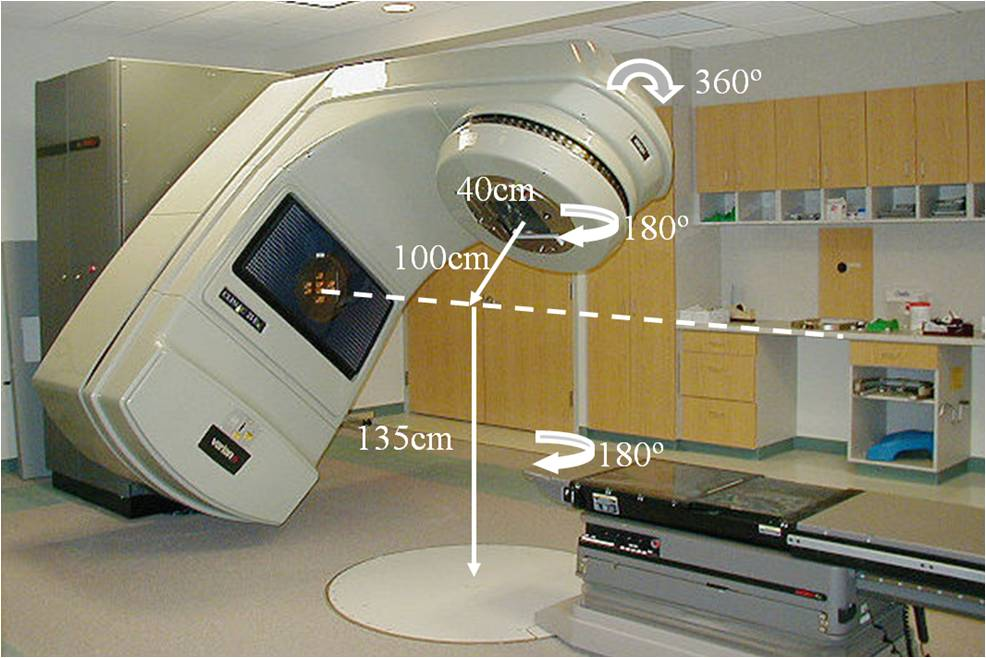
\includegraphics[width=100mm]{Acelerador2}
\caption[Exemplo de um acelerador linear utilizado no Hospital Universitário de Brasília.]{Exemplo de um acelerador linear utilizado no Hospital Universitário de Brasília. Os ângulos de 360${^{\textrm{o}} }$, 180${^{\textrm{o}} }$ e 180${^{\textrm{o}} }$ indicam os possíveis valores de rotação do acelerador e do \emph{gantry}. Os valores em centímetros indicam as dimensões do \emph{gantry} e as distâncias em relação à mesa e ao chão. Fonte:~\cite{Avelino2013}.}\label{fig:acelerador}
\end{figure}

Se você inserir figuras de outras fontes (livros, artigos, etc), deve incluir a fonte na legenda. Diga explicitamente ``Fonte: [X]'', sendo X a referência de onde foi tirada a figura. Ou use ``Adaptada de [X]'', caso a figura tenha sido modificada (por exemplo, traduzida). Não abuse, no entanto, da utilização de figuras de outras fontes. Dê preferência a trabalhos de sua autoria. Note que uma figura de outra fonte, mesmo com a devida citação, só poderia ser utilizada com autorização por escrito, para evitar processo por direitos autorais. Já o caso de inclusão de figuras de outras fontes sem a devida citação constitui plágio, sendo o autor do plágio sujeito à perda do título eventualmente obtido com a publicação e de outros direitos dela decorrentes.

\textbf{No caso de figuras de sua própria autoria, não indique isso na legenda. Não escreva, por exemplo, ``Fonte: o autor''}. Já se assume no texto que todo o material apresentado é produção do autor indicado, e os outros casos, que devem ser comparativamente poucos, é que devem ser explicitados.

\section{Observações Sobre Equações}

As equações são normalmente escritas de forma centralizada ao longo da direção horizontal, e com uma numeração à direita no caso das equações que são citadas. As equações que não são citadas posteriormente não precisam ser numeradas. Quando há numeração, ela aparece entre parênteses, e no formado x.y, com x o número do capítulo e y o número da equação dentro do capítulo.

Segue um exemplo de uma equação. Em um triângulo retângulo, a medida da hipotenusa é dada por
\begin{equation}\label{eq:hipotenusa}
a = \sqrt{b^2 + c^2},
\end{equation}
com ${b}$ e ${c}$ as medidas dos dois catetos.

Note em \eqref{eq:hipotenusa} que a equação faz parte do texto, no sentido de que ela não interrompe o fluxo da frase iniciada por ``Em um triângulo''. Não se deve, por exemplo, escrever ``a medida da hipotenusa é dada pela Equação 2.1'', e então colocar a equação abaixo como se fosse um objeto à parte do parágrafo (como acontece com as figuras e tabelas -- estas sim não se inserem no próprio texto, e são referenciadas como objetos independentes do parágrafo).

Por este motivo, as equações devem ser pontuadas conforme o texto normal. Elas devem ser seguidas, por exemplo, de ponto, vírgula, ou ponto-e-vírgula, conforme o fluxo do texto, a não ser que o texto imediatamente continue com a palavra ``e''.

Além disso, observe que todos os termos de uma equação que não foram previamente definidos devem ser definidos logo em seguida, como no caso de \eqref{eq:hipotenusa}. Os termos ${b}$ e ${c}$ foram definidos imediatamente após a equação. Nunca deve haver termos numa equação que não são explicitamente definidos no texto.

Segue um outro exemplo. A transformada discreta de Fourier de um sinal ${x}$ de comprimento ${N}$ é dada por
\begin{equation}
\hat{x}[k]=\sum_{n=0}^{N-1}x[n]\exp\left(-j\frac{2\pi nk}{N}\right),
\end{equation}
sendo ${j}$ a unidade imaginária e ${k}$ o índice de frequência considerado, com ${k\in\left\{0,1,\ldots,N\right\}}$.

\chapter{Materiais e Métodos}\label{chap:Metodologia}

Este capítulo pode ter outro nome, e na verdade sugiro um nome mais específico; indique no título sobre os tópicos metodológicos tratados. Pode ser usado mais de um capítulo para esses tópicos, se necessário.

Inclua as seções que se façam necessárias.

\section{Dicas para o capítulo}
Dicas importantes que devem ser contempladas neste capítulo, segundo~\cite{marconi.lakatos:2003}:
\begin{itemize}
\item Verificar se o capítulo responde as seguintes questões: Como? Com quê? Onde? Quanto?
\item A linguagem do projeto deve ser escrita com tempo verbal no futuro e da dissertação no passado.
\item É importante mencionar sobre: tipo de pesquisa (bibliográfica, descritiva, documental, experimental etc), dados (fonte de dados, forma de obtenção), população e amostra, tratamento e análise dos dados (descrição mais detalhada do método -- ou métodos -- que serão utilizados), limitações da pesquisa.
\end{itemize}

\section{Observações Sobre Quadros e Tabelas}

Quadros e tabelas são de uso semelhante às figuras, no que diz respeito à numeração, uso de legenda, e necessidade de citar ao menos uma vez antes da ocorrência. No entanto, no caso dos quadros e tabelas a legenda deve ser colocada acima, e não abaixo como nas figuras.

A Tabela~\ref{tab:exemplo} ilustra esse uso. Observe que a citação de uma tabela específica (pelo número) é com a palavra ``tabela'' em maiúscula, ao contrário da referência a tabelas em geral. Note que em uma tabela as bordas são horizontais (não use bordas verticais para separar colunas), e não são necessárias bordas para separar cada linha. Separe apenas as linhas do início, fim, e dos indicadores dos campos presentes, como no exemplo. Podem ser usadas bordas horizontais para separar regiões distintas de dados (seções de dados), se necessário.

\begin{table}[h]
\centering
\caption{Parâmetros utilizados na implementação do método de deteção de bordas proposto, em cada configuração considerada.}\label{tab:exemplo}
\begin{tabular}{ccllll}
\cline{1-5}
\multirow{2}{*}{Configuração} && \multicolumn{3}{l}{\hspace*{12pt}Parâmetro}&  \\
&& \hspace{4pt}A\hspace{4pt} & \hspace{4pt}B\hspace{4pt} & \hspace{4pt}C\hspace{4pt} & \\ \cline{1-5}
1                             && \hspace{4pt}10\hspace{4pt}        & \hspace{4pt}5\hspace{4pt}       & \hspace{4pt}2\hspace{4pt}       &  \\
2                             && \hspace{4pt}20\hspace{4pt}        & \hspace{4pt}5\hspace{4pt}       & \hspace{4pt}3\hspace{4pt}       &  \\
3                             && \hspace{4pt}30\hspace{4pt}        & \hspace{4pt}8\hspace{4pt}       & \hspace{4pt}5\hspace{4pt}       &  \\ \cline{1-5}
\end{tabular}
\end{table}

O Quadro~\ref{quadro:exemplo} é um outro exemplo. Note que um quadro se diferencia de uma tabela pelo uso de campos fechados, por meio de linhas horizontais e verticais. As tabelas são mais usadas para dados quantitativos, enquanto quadrados são mais usados quando há descrições textuais (mesmo que haja dados quantitativos também).

\begin{quadro}
\caption{Exemplo de um quadro (retirado de~\cite{Gomes2011}): \emph{Variáveis explicativas que representam características socioeconômicas dos idosos.} Fonte:~\cite{Gomes2011}}\label{quadro:exemplo}
\begin{center}
\scalefont{0.705}
\begin{tabular}{|l|l|l|}
\hline
\hfill Variável\hfill\hspace{1mm} & \hfill Descrição${^{*}}$\hfill\hspace{1mm} & \hfill Categorização\hfill\hspace{1mm}\\
\hline
Nível de escolaridade & Número de anos de estudo (A5a, A5b, A6) & \begin{tabular}{l}Nenhum\\1 a 7 anos\\8 anos e mais\end{tabular}\\
\hline
Tem seguro/plano privado de saúde?&\hspace{-06pt}\begin{tabular}{l}Que tipo de seguro de saúde o(a) Sr.(a)\\ tem? (F1)\end{tabular} & \begin{tabular}{l}Sim\\Não\end{tabular}\\
\hline
Tem casa própria?&Esta casa é: (J2) & \begin{tabular}{l}Sim\\Não\end{tabular}\\
\hline
Uso de serviços de saúde&\hspace{-06pt}\begin{tabular}{l}Durante os últimos 12 meses, aonde o(a)\\ Sr.(a) foi quando se sentiu doente ou quando\\ precisou fazer uma consulta de saúde? (F3)\end{tabular} & \begin{tabular}{l}Usou\\Não usou\end{tabular}\\
\hline
Estado nutricional&\hspace{-06pt}\begin{tabular}{l}Com relação a seu estado nutricional o(a) \\Sr.(a) se considera bem nutrido? (C22i)\end{tabular} & \begin{tabular}{l}Bem nutrido\\Não está bem nutrido\end{tabular}\\
\hline
\end{tabular}
\scalefont{1.4184}
\end{center}
\vspace{-12pt}
Fonte: Estudo SABE.\\
\emph{${^{\textrm{*} }}$Os códigos em parênteses na descrição das variáveis se referem à identificação da variável no banco de dados do Estudo SABE.}~\cite{Gomes2011}
\end{quadro}

\chapter{Resultados e Discussões}\label{chap:RD}

\begin{table}[h]
\centering
\caption{Fatores de qualidades medidos em função do número de amostras, nos testes de reconstrução realizados.}\label{tab:qualidade}
\begin{tabular}{cc}
\toprule
Número de amostras & Fator de qualidade\\
\midrule
10 & 0.30\\
20 & 0.45\\
30 & 0.60\\
40 & 0.90\\
50 & 0.93\\
\bottomrule
\end{tabular}
\end{table}

\begin{table}[h]
\centering
\caption{Outro exemplo de tabela.}\label{tab:outroexemplo}
\begin{tabular}{ccccc}
    \toprule
    a     & b     & c     & d     & e \\
    \midrule
    10    & 20    & 30    & 40    & 50 \\
    100   & 200   & 300   & 400   & 500 \\
    \bottomrule
    \end{tabular}%
\end{table}

\chapter{Conclusão}\label{chap:Conclusao}

\renewcommand\bibname{\Large\scshape Lista de Referências}
\addcontentsline{toc}{chapter}{\bf Lista de Referências}
\bibliography{referencias}

% |--- Exemplos de Apêndices ---|----------------------{{{
% Início do Apêndice
\newcounter{apendice}
\counterwithin{figure}{apendice}
\counterwithin{table}{apendice}
\renewcommand{\theapendice}{\Alph{apendice}}
\DeclareRobustCommand{\novoapendice}[1]{%
    \refstepcounter{apendice}%
    \phantom{\theapendice}\label{#1}}

% Exemplo 1
\clearpage
\begin{flushright}
\novoapendice{apendice_exemplo}
\scalebox{1.3}{\bfseries\scshape Apêndice~\ref{apendice_exemplo}}
\addcontentsline{toc}{chapter}{Apêndice~\ref{apendice_exemplo}}
\end{flushright}

\noindent\begin{large}{\bfseries\scshape Exemplo de Apêndice}\end{large} \label{sec:apendice1}

\vspace{24pt}

Se você desejar, pode incluir ao final um ou mais apêndices, e um ou mais anexos. Caso não queira, é só remover todo o conteúdo começando na linha marcada por ``\%~Início~do~Apêndice'', até a linha anterior a ``\verb|\end{document}|''.

% Exemplo 2
\clearpage
\begin{flushright}
\novoapendice{apendice_outro_exemplo}
\scalebox{1.3}{\bfseries\scshape Apêndice~\ref{apendice_outro_exemplo}}
\addcontentsline{toc}{chapter}{Apêndice~\ref{apendice_outro_exemplo}}
\end{flushright}

\noindent\begin{large}{\bfseries\scshape Outro Exemplo de Apêndice}\end{large} \label{sec:apendice2}

\vspace{24pt}

Se você desejar, pode incluir ao final um ou mais apêndices, e um ou mais anexos. Caso não queira, é só remover todo o conteúdo começando na linha marcada por ``\%~Início~do~Apêndice'', até a linha anterior a ``\verb|\end{document}|''.
%---}}}

% |--- Exemplos de Anexos ---|----------------------{{{
% Início do anexos
\newcounter{anexo}
\counterwithin{figure}{anexo}
\counterwithin{table}{anexo}
\renewcommand{\theanexo}{\Alph{anexo}}
\DeclareRobustCommand{\novoanexo}[1]{%
    \refstepcounter{anexo}%
    \phantom{\theanexo}\label{#1}}

% Exemplo 1
\clearpage
\begin{flushright}
\novoanexo{anexo_exemplo}
\scalebox{1.3}{\bfseries\scshape Anexo~\ref{anexo_exemplo}}
\addcontentsline{toc}{chapter}{Anexo~\ref{anexo_exemplo}}
\end{flushright}

\noindent\begin{large}{\bfseries\scshape Exemplo de Anexo}\end{large} \label{sec:anexo1}

\vspace{24pt}

Se você desejar, pode incluir ao final um ou mais apêndices, e um ou mais anexos. Caso não queira, é só remover todo o conteúdo começando na linha marcada por ``\%~Início~do~Apêndice'', até a linha anterior a ``\verb|\end{document}|''.

% Exemplo 2
\clearpage
\begin{flushright}
\novoanexo{anexo_outro_exemplo}
\scalebox{1.3}{\bfseries\scshape Anexo~\ref{anexo_outro_exemplo}}
\addcontentsline{toc}{chapter}{Anexo~\ref{anexo_outro_exemplo}}
\end{flushright}

\noindent\begin{large}{\bfseries\scshape Outro Exemplo de Anexo}\end{large} \label{sec:anexo2}

\vspace{24pt}

Se você desejar, pode incluir ao final um ou mais apêndices, e um ou mais anexos. Caso não queira, é só remover todo o conteúdo começando na linha marcada por ``\%~Início~do~Apêndice'', até a linha anterior a ``\verb|\end{document}|''.
%---}}}

\end{document} 
%---}}}
